\documentclass{beamer}
\usetheme{TTU}
\usefonttheme{serif}
\usepackage[T1]{fontenc}
\usepackage[utf8]{inputenc}
\usepackage{mathptmx}
\usepackage{url}
\usepackage{graphicx}
\usepackage{setspace}
\usepackage{esint}
\usepackage[natbibapa]{apacite}
\usepackage{color}
\usepackage{amsmath}
\usepackage{amsfonts}
\usepackage{bm}
\usepackage{Sweavel}
\usepackage{listings}

\def\Sweavesize{\scriptsize}
\def\Rcolor{\color{black}}
%\def\Routcolor{\color{red}}
\def\Rcommentcolor{\color{violet}}
\def\Rbackground{\color[gray]{0.85}}
\def\Routbackground{\color[gray]{0.85}}

\lstset{tabsize=2, breaklines=true, style=Rstyle}



\newcommand{\red}[0]{\textcolor{red}}
%\newcommand{\violet}[0]{\textcolor{violet}}
\newcommand{\green}[0]{\textcolor{green}}
\newcommand{\blue}[0]{\textcolor{blue}}
\newcommand{\comment}[1]{}
\newcommand{\kfold}[0]{\emph{K}-fold cross-validation}

\title[Lecture 5]{Lecture 5: More Nuts and Bolts---FIML and Categorical Data MI}
\subtitle{EPSY 6349: Modern Missing Data Analysis}

\author{Kyle M. Lang}

\institute[TTU IMMAP]{
  Institute for Measurement, Methodology, Analysis \& Policy\\
  Texas Tech University\\
  Lubbock, TX
}

\date{September 29, 2015}


\begin{document}

\setkeys{Gin}{width=\textwidth}

\input{sweaveFiles/lecture5-001}


% Use a custom background template for the title slide
{\usebackgroundtemplate{\rule{0pt}{3.4in}\hspace*{2.25in}
    \makebox[0pt][r]{
\includegraphics[natwidth=1000bp, natwidth=283bp,width=2in]{TTU_Logo.png}}}

  \begin{frame}[plain]

    \titlepage

  \end{frame}
}% CLOSE Custom Background Template



\begin{frame}{Outline}

  \begin{itemize}
  \item Look at FIML in more depth
    \vspace{12pt}
    \begin{itemize}
    \item Show how to do ML and FIML (semi) by hand in \textsf{R}.
    \end{itemize}
    \vspace{12pt}
  \item Discuss MI for categorical variables.
    \vspace{12pt}
    \begin{itemize}
    \item Show a manual \textsf{R} example.
    \end{itemize}
  \end{itemize}

\end{frame}


\begin{frame}{FIML Conceptual Refresher}

  FIML is an ML estimation method that is robust to ignorable
  nonresponse.\\
  \vspace{12pt}
  FIML partitions the missing information out of the
  likelihood function so that the model is only estimated from the
  observed parts of the data.\\
  \vspace{12pt}
  After a minor alteration to the likelihood function,
  FIML reduces to simple ML estimation.\\
  \vspace{12pt}
  So, let's review ML estimation before moving forward.

\end{frame}


\begin{frame}[shrink = 5]{Maximum Likelihood Estimation Refresher}

  ML estimation simply finds the parameter values that are ``most
  likely'' to have given rise to the observed data.
  \vspace{6pt}
  \begin{itemize}
    \item The \emph{likelihood} function is just a probability density
      (or mass) function with the data treated as fixed and the
      parameters treated as random variables.
    \vspace{6pt}
    \item Having such a framework allows us to ask: ``Given that I've
      observed these data values, what parameter values most probably
      describe these data?''
  \end{itemize}
  \vspace{12pt}
  \pause
  ML estimation is usually employed when there is no closed form
  solution for the parameters we seek.
  \begin{itemize}
    \item This is why you don't usually see ML used to fit OLS
      regression models or ordinary ANOVAs.
  \end{itemize}
  \vspace{12pt}
  After choosing a likelihood function, we iteratively
  optimize the function to produce the ML estimated parameters.
  \begin{itemize}
  \item In practice, we nearly always work with the natural logarithm
    of the likelihood function (i.e., the \emph{loglikelihood}).
  \end{itemize}

\end{frame}


\begin{frame}{Steps of ML}

  \begin{enumerate}
    \item Choose a loglikelihood function $f(X|\theta)$ to describe
      the distribution of the data given the parameters.
      \vspace{6pt}
    \item Choose some initial estimate of $\theta$, $\hat{\theta}^{(0)}$.
      \vspace{6pt}
    \item Compute each row's value for the likelihood function
      parameterized by $\hat{\theta}$, $f(x_n|\hat{\theta})$.
      \vspace{6pt}
    \item Sum the individual loglikelihood value into the joint
      loglikelihood of the data: $LL = \sum_{n = 1}^N
      f(x_n|\hat{\theta})$.
      \vspace{6pt}
    \item Choose a ``better'' estimate of the parameters
      $\hat{\theta}^{(1)}$ and repeat steps 3 and 4.
      \vspace{6pt}
    \item Repeat steps 3 -- 5 until the change between $LL^{(i)}$ and
      $LL^{(i + 1)}$ is negligible.
      \vspace{6pt}
    \item Take $\hat{\theta}^{(i)}$ as your estimated parameters.
  \end{enumerate}

\end{frame}


\begin{frame}{ML Example}

  Recall the multivariate normal loglikelihood function:
  \begin{align*}
    \textit{LL}_n = -\frac{P}{2} \ln(2\pi) - \frac{1}{2} \ln | \Sigma
    | - \frac{1}{2} (\mathbf{Y}_n - \mu)^T \Sigma^{-1}(\mathbf{Y}_n -
    \mu) \label{llEq}
  \end{align*}

  \vspace{12pt}

  We can define this function manually in \textsf{R}:

\begin{Schunk}
\begin{Sinput}
 ## Row i's contribution to the overall LL:
 llVec[i] <- -0.5 * nVar * log(2 * pi) -
     0.5 * log(det(sigmaHat)) -
         0.5 * (inData[i, ] - muHat) %*%
             solve(sigmaHat) %*%
                 matrix(inData[i, ] - muHat)
\end{Sinput}
\end{Schunk}


\end{frame}


\begin{frame}{ML Example}

  We can wrap the preceding code in an \textsf{R} function that takes
  a parameter vector and a data set and returns the total loglikelihood
  value for the data:

\begin{Schunk}
\begin{Sinput}
 ## Complete data loglikelihood function:
 myLL <- function(parVec, inData)
 {
     ## Extract the parameter matrices:
     nVar <- ncol(inData)
     muHat <- parVec[1 : 3]
     sigmaHat <- matrix(parVec[4 : 12], ncol = 3)
 
     ## Compute the row-wise LogLikelihoods:
     llVec <- rep(NA, nrow(inData))
     for(i in 1 : nrow(inData)) {
         llVec[i] <- -0.5 * nVar * log(2 * pi) -
             0.5 * log(det(sigmaHat)) -
                 0.5 * (inData[i, ] - muHat) %*%
                     solve(sigmaHat) %*%
                         matrix(inData[i, ] - muHat)
     }
     sum(llVec)# return the overall LL value
 }
\end{Sinput}
\end{Schunk}


\end{frame}


\begin{frame}[allowframebreaks]{ML Example}
  The \textbf{optimx} package in R can numerically optimize arbitrary
  functions. We can use it to do ML by hand.

\begin{Schunk}
\begin{Sinput}
 parms <- list()
 parms$nObs <- 1000
 parms$meanVec <- c(1.0, 2.0, 3.0)# x, y, z
 parms$corVec <- c(0.2, 0.5, 0.4)# xy, xz, yz
 ## Create some toy data:
 simData <- simulateSimpleData(parms)
 ## Vector of starting values for the parameters:
 startVec <- c(rep(0.5, 3),
               c(1.0, 0.3, 0.3,
                 0.3, 1.0, 0.3,
                 0.3, 0.3, 1.0))
 ## Use optimx() to numerically optimize the LL function:
 llOpt <- optimx(startVec,
                 fn = myLL,
                 inData = as.matrix(simData),
                 method = "L-BFGS-B",
                 lower = 0.0,
                 control = list(maximize = TRUE,
                     kkt = FALSE))
\end{Sinput}
\begin{Soutput}
Maximizing -- use negfn and neggr
\end{Soutput}
\begin{Sinput}
 ## Get the optimize mean vector and covariance matrix:
 muHatLL <- llOpt[1 : 3]
 sigmaHatLL <- matrix(as.numeric(llOpt[4 : 12]), ncol = 3)
 ## Look at the results:
 muHatLL
\end{Sinput}
\begin{Soutput}
               p1       p2       p3
L-BFGS-B 1.033976 1.985203 3.009896
\end{Soutput}
\begin{Sinput}
 sigmaHatLL
\end{Sinput}
\begin{Soutput}
          [,1]      [,2]      [,3]
[1,] 1.0125147 0.1805506 0.4952722
[2,] 0.1805501 0.9265573 0.3427037
[3,] 0.4952725 0.3427032 0.9519676
\end{Soutput}
\end{Schunk}


\pagebreak

\begin{Schunk}
\begin{Sinput}
 muHatLL - colMeans(simData)
\end{Sinput}
\begin{Soutput}
                   p1            p2            p3
L-BFGS-B 2.984267e-06 -7.713401e-06 -6.986144e-06
\end{Soutput}
\begin{Sinput}
 sigmaHatLL - cov(simData)
\end{Sinput}
\begin{Soutput}
              x             y             z
x -0.0010179749 -0.0001840542 -0.0005330290
y -0.0001845228 -0.0009284928 -0.0003518237
z -0.0005327091 -0.0003522739 -0.0009734289
\end{Soutput}
\end{Schunk}


\end{frame}


\begin{frame}{FIML Example}

  We can do this same process for FIML estimation.\\
  \vspace{12pt}
  Recall the FIML loglikelihood function:
   \begin{align*}
    \textit{LL}_{\textit{FIML,n}} = -\frac{P}{2} \ln(2\pi) -
    \frac{1}{2} \ln | \Sigma_n | - \frac{1}{2} (\mathbf{Y}_n -
    \mu_n)^T \Sigma_n^{-1}(\mathbf{Y}_n - \mu_n)
  \end{align*}

   \vspace{12pt}

   We can also define this version manually in \textsf{R}:

\begin{Schunk}
\begin{Sinput}
 ## Subset mu, sigma, and inData to only work
 ## with the observed parts of inData:
 isObs <- !is.na(inData[i, ])
 nVar <- sum(isObs)
 llVec[i] <- -0.5 * nVar * log(2 * pi) -
     0.5 * log(det(sigmaHat[isObs, isObs])) -
         0.5* (inData[i, isObs] - muHat[isObs]) %*%
             solve(sigmaHat[isObs, isObs]) %*%
                 matrix(inData[i, isObs] - muHat[isObs])
\end{Sinput}
\end{Schunk}


\end{frame}


\begin{frame}[shrink = 10]{FIML Example}

  Construct a wrapper function to get the overall LL value:

\begin{Schunk}
\begin{Sinput}
 ## FIML loglikelihood function:
 myFIML <- function(parVec, inData)
 {
     ## Extract the parameter matrices:
     nVar <- ncol(inData)
     muHat <- parVec[1 : 3]
     sigmaHat <- matrix(parVec[4 : 12], ncol = 3)
 
     ## Compute the row-wise -2LogLikelihoods:
     llVec <- rep(NA, nrow(inData))
     for(i in 1 : nrow(inData)) {
         ## Subset mu, sigma, and inData to only work
         ## with the observed parts of inData:
         isObs <- !is.na(inData[i, ])
         nVar <- sum(isObs)
 
         llVec[i] <- -0.5 * nVar * log(2 * pi) -
             0.5 * log(det(sigmaHat[isObs, isObs])) -
                 0.5 * (inData[i, isObs] - muHat[isObs]) %*%
                     solve(sigmaHat[isObs, isObs]) %*%
                         matrix(inData[i, isObs] - muHat[isObs])
     }
     sum(llVec) # return the overall LL value
 }
\end{Sinput}
\end{Schunk}


\end{frame}


\begin{frame}[allowframebreaks]{FIML Example}

  And we can use \textbf{optimx} to numerically optimize the FIML
  objective:

\begin{Schunk}
\begin{Sinput}
 parms$pm <- 0.3
 parms$auxVar <- "z"
 parms$incompVars <- "y"
 parms$marType <- "lower"
 # Impose missing data on the toy data:
 missData <- imposeMissing(simData, parms)
 ## Use optimx() to numerically optimize the FIML objective:
 fimlOpt <- optimx(startVec,
                   fn = myFIML,
                   inData = as.matrix(missData),
                   method = "L-BFGS-B",
                   lower = 0.0,
                   control = list(maximize = TRUE,
                       kkt = FALSE))
\end{Sinput}
\begin{Soutput}
Maximizing -- use negfn and neggr
\end{Soutput}
\begin{Sinput}
 ## Get the optimized mean vector and covariance matrix:
 muHatFIML <- as.numeric(fimlOpt[1 : 3])
 sigmaHatFIML <-
     matrix(as.numeric(fimlOpt[4 : 12]), ncol = 3)
 ## Look at the results:
 muHatFIML
\end{Sinput}
\begin{Soutput}
[1] 1.033963 1.945265 3.009926
\end{Soutput}
\begin{Sinput}
 sigmaHatFIML
\end{Sinput}
\begin{Soutput}
          [,1]      [,2]      [,3]
[1,] 1.0125127 0.1896069 0.4953259
[2,] 0.1896089 0.9016940 0.3807157
[3,] 0.4953237 0.3807173 0.9519759
\end{Soutput}
\end{Schunk}


\end{frame}


\begin{frame}[allowframebreaks]{FIML Example}

  Just to make sure our results are plausible, we can do the same
  analysis using lavaan():

\begin{Schunk}
\begin{Sinput}
 ## Confirm the manual approach by using
 ## lavaan() to get the FIML estimates:
 mod1 <- "
 x ~~ y + z
 y ~~ z
 "
 ## Fit the model with lavaan():
 out1 <- cfa(mod1, data = missData, missing = "fiml")
 muHatFIML2 <- inspect(out1, "est")$nu
 sigmaHatFIML2 <- inspect(out1, "theta")
\end{Sinput}
\end{Schunk}


\pagebreak

\begin{Schunk}
\begin{Sinput}
 ## Same as what we got by hand :)
 sigmaHatFIML - sigmaHatFIML2
\end{Sinput}
\begin{Soutput}
  x y z
x 0 0 0
y 0 0 0
z 0 0 0
\end{Soutput}
\begin{Sinput}
 muHatFIML - muHatFIML2
\end{Sinput}
\begin{Soutput}
  intrcp
x      0
y      0
z      0
\end{Soutput}
\end{Schunk}


\end{frame}


\begin{frame}

  \begin{center}
    \textsc{\huge{Categorical Variable MI}}
  \end{center}

\end{frame}


\begin{frame}{Orienting Categorical Variable MI}

  As we've seen, MI is basically just a slightly more complicated flavor
  of out-of-sample prediction using regression.
  \vspace{6pt}
  \begin{itemize}
  \item So far, we've only considered imputation using linear regression
    models.
    \vspace{6pt}
  \item What do we need to modify to address categorical outcomes?
    \vspace{6pt}
    \begin{itemize}
    \item Can we use OLS for prediction with categorical DVs?
    \end{itemize}
  \end{itemize}

\end{frame}


\begin{frame}{Motivating the Generalized Linear Model}

  OLS regression is a type of \emph{General Linear Model}.
  \vspace{6pt}
  \begin{itemize}
  \item A normally distributed outcome variable is linearly associated
    with a set of predictor variables (which may be non-linear
    transformations of the observed predictors)
  \end{itemize}
  \vspace{12pt}
  Generalized Linear Models take the form:
  \begin{align*}
    Y &= \mathbf{X}\beta + \varepsilon\\
    &\text{with } \varepsilon = Y|\mathbf{X} \sim \text{N}(\mu, \sigma^2)
  \end{align*}
  If we have a binary outcome, for example, we can't simply assume it
  follows a normal distribution and model it as the linear combination
  of some predictors.
  \vspace{6pt}
  \begin{itemize}
  \item Why not?
  \end{itemize}

\end{frame}


\begin{frame}{Overview of the Generalized Linear Model}

  The \emph{Generalized Linear Model} is an extension of the General
  Linear Model that allows the DV to follow non-normal distributions.
  \vspace{6pt}
  \begin{itemize}
  \item Most importantly, the Generalized Linear Model allows for
    discrete distributions of the DV
  \end{itemize}
  \vspace{12pt}
  Generalized Linear Models take the form:
  \begin{align*}
    g(\mu_Y) &= \mathbf{X}\beta\\
             &\text{with } Y | \mathbf{X} \sim f(Y | \mu, \phi)
  \end{align*}
  Some terminology:
  \begin{itemize}
  \item $\mathbf{X}\beta$ is called the \emph{Systematic Component}
  \item $f(Y | \mu, \phi)$ is called the \emph{Random Component}
  \item $g(\cdot)$ is called the \emph{Link Function}
    \begin{itemize}
    \item $g^{-1}(\cdot)$ is sometimes called the \emph{Activation
        Function}.
    \end{itemize}
  \end{itemize}

\end{frame}


\begin{frame}{Parts of the Generalized Linear Model}

  The systematic component is simply the weighted sum of the predictors
  \begin{itemize}
  \item Exactly the same as in OLS regression
  \end{itemize}
  \vspace{12pt}
  \pause
  The random component is the (conditional) distribution of the outcome
  after accounting for the systematic component.
  \begin{itemize}
  \item In OLS regression, the systematic component is the normal
    distribution
  \item Logistic and Probit regression use the \emph{Binomial
      Distribution} as their random component.
  \end{itemize}

\end{frame}


\begin{frame}{Parts of the Generalized Linear Model}

  The link function ``linearizes'' the outcome variable, so that it
  can be modeled by the systematic component.
  \begin{itemize}
  \item OLS regression uses the so-called \emph{Identity Link}:
    \begin{align*}
      g(\mu_Y) = \mu_Y.
    \end{align*}
    \vspace{6pt}
  \item Logistic regression uses the \emph{Logit Link}:
    \begin{align*}
      g(\mu_Y) = \ln \left\{ \frac{P(y = 1 | \mathbf{X})}{(1 - P(y = 1
      | \mathbf{X}))} \right\},
    \end{align*}
    which represents the log-odds of success on Y.
    \vspace{12pt}
  \item Probit regression uses the \emph{Probit Link}:
    \begin{align*}
      \mu_Y = \Phi(\mathbf{X}\beta) \Rightarrow g(\mu_Y) =
      \Phi^{-1}(\mathbf{X}\beta),
    \end{align*}
    which returns the quantile on the standard normal CDF associated
    with each value of the systematic component.
  \end{itemize}

\end{frame}


\begin{frame}{Latent Variable Representation of GLMs}

  GLMs are usually fit directly to the discrete data using marginal ML
  or iteratively reweighted least squares.\\
  \vspace{12pt}
  Many GLMs, however, can be formulated in terms of unobserved
  \emph{Latent Response Indicators}.
  \begin{itemize}
  \item If we assume that our observed, discrete outcome is an
    imperfect coarsening of an underlying continuous variable, we
    can model the unobserved continuous variable.
  \end{itemize}
  \vspace{12pt}
  Probit Regression already implicitly assumes a latent response
  indicator. It's latent formulation takes the form:
  \begin{align*}
    Y^* &= \mathbf{X}\beta + \varepsilon\\
    Y &= \left\{ \begin{array}{ccl}
                   1 & \text{when} & Y^* > 0\\
                 0 & \text{when} & Y^* \leq 0
                 \end{array}\right.
  \end{align*}

\end{frame}


\begin{frame}{Why do we care?}

  The latent variable representations of GLMs can dramatically simplify
  Bayesian modeling of some GLMs.\\
  \vspace{12pt}
  Due to the simple formulate shown above, we can construct the
  following Bayesian Probit Model:
  \begin{align*}
    Y^* &\sim \left\{
          \begin{array}{ccl}
            \text{Trunc-N}^+(\mathbf{X}\beta, ~ \mathbf{1}) & \text{when}
            & Y = 1\\
            \text{Trunc-N}^-(\mathbf{X}\beta, ~ \mathbf{1}) & \text{when}
            & Y = 0
          \end{array}\right.\\
    \\
    \beta &\sim \text{N} \left( (\mathbf{X}^T \mathbf{X})^{-1}
            \mathbf{X}^T Y^*, ~ (\mathbf{X}^T \mathbf{X})^{-1} \right)\\
    \\
    Y &= \left\{ \begin{array}{ccl}
                   1 & \text{when} & Y^* > 0\\
                   0 & \text{when} & Y^* \leq 0
                 \end{array}\right.
  \end{align*}

\end{frame}


\begin{frame}{Creating Imputations from the Latent Probit Model: Model
    Estimation}

  \begin{enumerate}
  \item Start with an initial guess of $Y^{*(0)}$.
    \vspace{6pt}
  \item Regress $Y^{*(0)}$ onto $\mathbf{X}_{obs}$ to get
    $\hat{\beta}^{(0)}=(\mathbf{X}^T \mathbf{X})^{-1} \mathbf{X}^T Y^{*(0)}$
    \vspace{6pt}
  \item Use $\hat{\beta}^{(0)}$ to parameterize $P(\beta | Y^*,
    \mathbf{X})$
    \vspace{6pt}
  \item Sample a new vector of coefficients $\hat{\beta}^{(1)}$ from
    $P(\beta | Y^*, \mathbf{X})$.
    \vspace{6pt}
  \item Use $\hat{\beta}^{(1)}$ to compute $\mathbf{X}\beta$ and
    parameterize $P(Y^* | \beta, \mathbf{X})$.
    \vspace{6pt}
  \item Sample $Y^{*(1)}$ from $P(Y^* | \beta, \mathbf{X})$.
    \vspace{6pt}
  \item Repeat steps 2--6 until the model converges.
  \end{enumerate}

\end{frame}


\begin{frame}{Creating Imputations from the Latent Probit Model:
    Drawing Imputations}

  \begin{enumerate}
  \item Randomly sample $M$ sets of parameters $\beta^{(m)}$ from the
    stationary $P(\beta | Y^*, \mathbf{X})$
    \vspace{6pt}
  \item For each $\beta^{(m)}$ compute $Y_{mis}^{*(m)} =
    \mathbf{X}_{mis} \beta^{(m)}$
    \vspace{6pt}
  \item Calculate the predicted probabilities or success
    $P(Y = 1 | \mathbf{X}) = \Phi(Y^{*(m)})$ associated with each
    $Y^{*(m)}$
    \vspace{6pt}
  \item Compare the $P(Y = 1 | \mathbf{X})$ to a standard uniform
    variate $u_i$.
    \vspace{6pt}
  \item Create the imputations as follows:
    \begin{align*}
      Y_{imp} = \left\{ \begin{array}{ccl}
                          1 & \text{when} & P(Y = 1 | \mathbf{X}) > u_i\\
                          0 & \multicolumn{2}{l}{\text{otherwise}}
                        \end{array}\right.
    \end{align*}
  \end{enumerate}

\end{frame}


\begin{frame}[allowframebreaks]{Bayesian Probit Example}

\begin{Schunk}
\begin{Sinput}
 nReps <- 5000
 nImps <- 100
 ## Simulate some data:
 simData <- simulateSimpleData(parms)
 ## Categorize Y:
 simData[ , "y"] <- as.numeric(cut(simData[ , "y"], 2)) - 1
 ## Impose missing:
 missData <- imposeMissing(simData, parms)
 ## Subset the data:
 yMis <- missData[is.na(missData[ , "y"]), ]
 yObs <- missData[!is.na(missData[ , "y"]), ]
 ## Get some useful summaries:
 ySuccess <- yObs[ , "y"] == 1
 predMat <- as.matrix(cbind(1, yObs[ , c("x", "z")]))
 nObs <- nrow(yObs)
 ## Start the Gibbs sampled parameters:
 yStar <- rnorm(nObs)
 startFit <- lm.fit(y = yStar, x = predMat)
 coefs <- startFit$coef
 yHats <- startFit$fitted
 coefVar <- solve(crossprod(predMat))
\end{Sinput}
\end{Schunk}


\pagebreak

\begin{Schunk}
\begin{Sinput}
 ## Sample the posterior imputation model parameters:
 coefSams <- matrix(NA, nReps, length(coefs))
 for(rp in 1 : nReps) {
     ## Sample the latent response indicators:
     yStar[ySuccess] <- rtnorm(sum(ySuccess),
                               mean = yHats[ySuccess],
                               sd = 1.0,
                               lower = 0)
     yStar[!ySuccess] <- rtnorm(sum(!ySuccess),
                                mean = yHats[!ySuccess],
                                sd = 1.0,
                                upper = 0)
 
     ## Sample the regression coefficients:
     coefMean <- .lm.fit(y = yStar, x = predMat)$coef
     coefs <- matrix(rmvnorm(1, coefMean, coefVar))
     yHats <- predMat %*% coefs
 
     ## Store the coefficient samples for later:
     coefSams[rp, ] <- coefs
 }
\end{Sinput}
\end{Schunk}


\end{frame}


\begin{frame}{Posterior Parameter Distributions}

\input{sweaveFiles/lecture5-013}
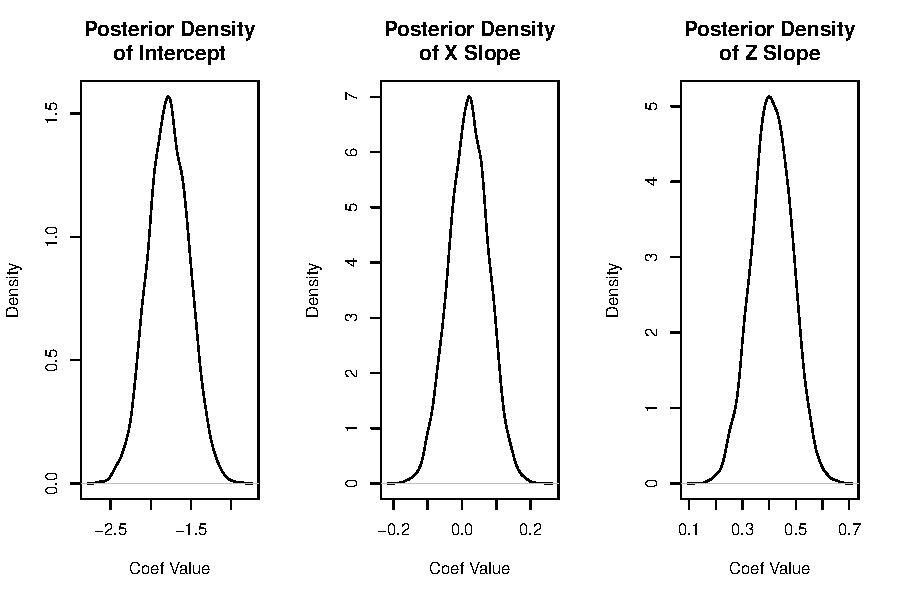
\includegraphics{sweaveFiles/lecture5-013}

\end{frame}


\begin{frame}{Create Imputations}

\begin{Schunk}
\begin{Sinput}
 ## Create the imputations:
 sampleIndex <- sample(c(1 : nReps), nImps)
 predMat <- as.matrix(cbind(1, yMis[ , c("x", "z")]))
 nObs <- nrow(yMis)
 impList <- list()
 counter <- 0
 for(m in sampleIndex) {
     counter <- counter + 1
 
     ## 1) Compute the predicted values on the z-scale
     ## 2) Convert these values to predicted probabilities
     ## 3) Check if each predictive probability exceeds
     ##    a standard uniform variate.
     ## 4) If 'yes' to (3) impute a 1, else impute a 0
     yHats <- predMat %*% coefSams[m, ]
     imps <- as.numeric(pnorm(yHats) >= runif(nObs))
 
     ## Fill the missing data with the imputations:
     impList[[counter]] <- missData
     impList[[counter]][is.na(missData[ , "y"]), "y"] <- imps
 }
\end{Sinput}
\end{Schunk}


\end{frame}


\begin{frame}{Same Idea with \textbf{mice}}

\begin{Schunk}
\begin{Sinput}
 ## Try the analogous process in mice():
 missData2 <- as.data.frame(missData)
 missData2$y <- factor(missData2$y)
 ## Create the imputations:
 miceOut <- mice(missData2,
                 m = nImps,
                 method = "logreg",
                 maxit = 10,
                 printFlag = FALSE)
 ## Fill the missing data with the imputations:
 impList2 <- list()
 for(m in 1 : nImps) impList2[[m]] <- complete(miceOut, m)
\end{Sinput}
\end{Schunk}


\end{frame}


\begin{frame}[allowframebreaks]{Fit the analysis models}

\begin{Schunk}
\begin{Sinput}
 ## Fit the analysis model to each imputation:
 fitList <- lapply(impList,
                   FUN = function(impData) {
                       glm(y ~ x + z,
                           data = as.data.frame(impData),
                           family = binomial("probit"))
                   })
 ## Fit the analysis models to mice's imputed data:
 fitList2 <- lapply(impList2,
                    FUN = function(impData) {
                        glm(y ~ x + z,
                            data = as.data.frame(impData),
                            family = binomial("probit"))
                    })
 ## Fit the complete data models:
 glmOut <- glm(y ~ x + z,
               data = as.data.frame(simData),
               family = binomial("probit"))
\end{Sinput}
\end{Schunk}


\pagebreak

\begin{Schunk}
\begin{Sinput}
 ## Compare the results:
 coef(MIcombine(fitList)) # By Hand
\end{Sinput}
\begin{Soutput}
(Intercept)           x           z 
-1.75928476  0.01737044  0.40571166 
\end{Soutput}
\begin{Sinput}
 coef(MIcombine(fitList2)) # With mice()
\end{Sinput}
\begin{Soutput}
(Intercept)           x           z 
-1.74696283  0.01144854  0.40399215 
\end{Soutput}
\begin{Sinput}
 coef(glmOut) # Using complete data
\end{Sinput}
\begin{Soutput}
(Intercept)           x           z 
-1.72581523  0.01980291  0.39418676 
\end{Soutput}
\end{Schunk}


\end{frame}


\begin{frame}{General MI Framework}

  Almost any proper implementation of MI amounts to out-of-sample
  prediction using a Bayesian generalized linear model. So, specifying
  an MI model will entail three steps:
  \vspace{6pt}
  \begin{enumerate}
  \item Choose a random component
    \begin{itemize}
    \item The distribution assumed for the missing data.
    \end{itemize}
    \vspace{6pt}
  \item Choose a systematic component
    \begin{itemize}
    \item The predictors of the imputation model
    \end{itemize}
    \vspace{6pt}
  \item Choose a link function
    \begin{itemize}
    \item The transformation linking the systematic component to the mean
      of the random component
    \item Often chosen hand-in-hand with the random component
    \end{itemize}
  \end{enumerate}
  \vspace{6pt}
  Each step in this process carries its own challenges.

\end{frame}


\begin{frame}{The End}

  \begin{center}
    \huge{Okay, let's talk term projects!}
  \end{center}

\end{frame}


\end{document}
